\section{Família Quadrática}

%--------------------

\begin{frame}
\vspace{5pt}
\frametitle{Família Quadrática}
\begin{columns}
\column{\dimexpr\paperwidth-15pt}

Considerar a família de funções $h: \RR \to \RR$ dadas por
$$h(x) = \mu x(1-x),$$
onde $\mu > 1$.
Essa família de funções é conhecida por família quadrática.

\begin{figure}[!htb]
\centering
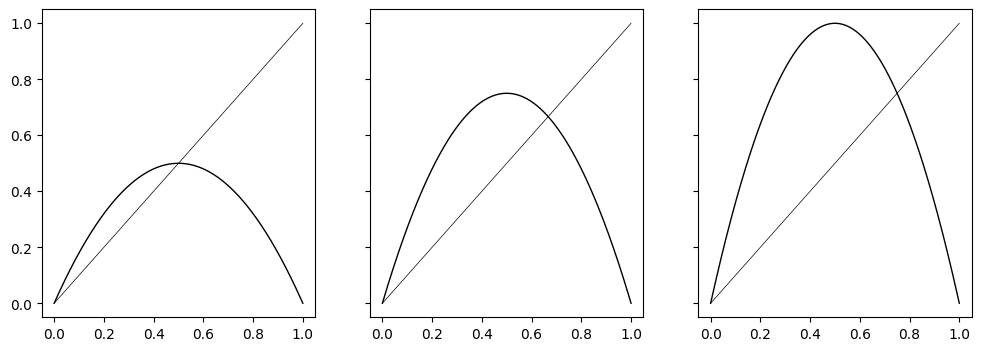
\includegraphics[scale=0.4]{images/h_2,3,4,5.png}
\caption{Gráficos de $h$ para $\mu = 2$, $\mu = 3$ e $\mu = 4$.}
\end{figure}

\end{columns}
\end{frame}
